\documentclass[11pt,a4paper]{article}
\usepackage[T1]{fontenc}
\usepackage[margin=2.3cm]{geometry}
\usepackage{amsmath,amssymb}
\usepackage{graphicx}
\usepackage[dvipsnames]{xcolor}
\usepackage{enumitem}
\usepackage[colorlinks=true,linkcolor=blue,urlcolor=blue]{hyperref}
\setlength{\parskip}{0.6em}
\setlength{\parindent}{0pt}
\begin{document}

\begin{center}{\LARGE\bfseries openheights}\\[0.4em]{\large Measure a tower or a tree with trigonometry and a phone, in three sessions.}\\[0.2em]\small PAN IIT OSS explainer \textbullet{} secondary school to diploma / undergraduate (levels 3-5)\end{center}

\section*{Why this exists}
Heights you cannot reach are found with angles and distances. This explainer shows the trigonometry of shadows and angles of elevation, and then something just as important: how a small error in an angle becomes an error in the height, and how to keep it small.

\section*{The end goal}
Measure the height of a tower or tree with trigonometry and a phone. The end goal is to measure the height of a tower or a tree with trigonometry and a phone, and to say how sure you are. The same ideas drive surveying, mapping and every measurement that mixes angles and lengths.

\section*{How the three sessions build up}
\begin{enumerate}[nosep]
\item \textbf{Session 1: Similar triangles, shadows and one angle} (Level 1, conceptual interactive model, 60 min).
\item \textbf{Session 2: Two angles, and how reading errors spread} (Level 2, mathematical engineering model, 75 min).
\item \textbf{Session 3: Simulating noisy readings, hills and averages} (Level 3, simulation and validation, 90 min).
\end{enumerate}

\section{Session 1: Similar triangles, shadows and one angle}

\subsection*{A. Real-world problem}
You cannot climb a tower or a tree with a tape measure, but you can stand on the ground. Two everyday tricks give the height: the shadow it casts, and the angle you tilt your head (or phone) to see its top. Why do these work, and what do you need to know about the ground?

\subsection*{B. Concept and theory}
Two triangles with the same angles are similar: their sides are in the same ratio. At one moment the sun makes the same angle with the ground everywhere, so a stick and a tower with their shadows form similar triangles, and height / shadow is the same for both. The angle of elevation a is measured from the horizontal at your eye up to the top. In the right triangle with horizontal side d and vertical side H above your eye, tan(a) = H / d, so H = d tan(a). The tower is higher than your eye by that amount, so you add your eye height to get the total height. This is a simplified model: flat ground, a vertical tower, a perfectly level phone and an exact distance.

\begin{itemize}[nosep]
\item h\_t, s\_t: tower height and its shadow length (m)
\item h\_s, s\_s: stick height and its shadow length (m)
\item d: horizontal distance from you to the base (m)
\item a: angle of elevation to the top (degrees)
\item e: eye height above the ground (m)
\item h: total height of the tower (m)
\end{itemize}

\begin{equation*}
\frac{h_t}{s_t}=\frac{h_s}{s_s}\quad\Rightarrow\quad h_t=h_s\,\frac{s_t}{s_s}
\end{equation*}

\begin{equation*}
\tan a=\frac{h-e}{d}
\end{equation*}

\begin{equation*}
h=d\tan a+e
\end{equation*}

\begin{center}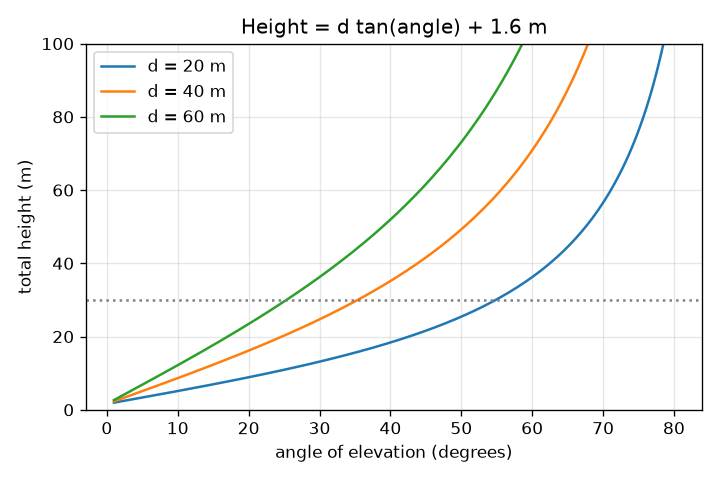
\includegraphics[width=0.85\linewidth]{figures/s01_height_vs_angle.png}\\\small Total height against angle for three distances: the tangent curve gets steeper at large angles.\end{center}

\subsection*{E. Worked example}
(a) A 1.5 m stick casts a 1.0 m shadow when a tower casts an 18 m shadow. How tall is the tower? (b) You stand 40 m from another tower, read 35 degrees, and your eye is 1.6 m high. How tall is it?
\begin{enumerate}[nosep]
\item (a) Ratio stick: 1.5 / 1.0 = 1.5 m of height per metre of shadow.
\item (a) Tower: 1.5 x 18 = 27 m.
\item (b) tan 35 degrees = 0.7002.
\item (b) Height above the eye = 40 x 0.7002 = 28.01 m.
\item (b) Total = 28.01 + 1.6 = 29.61 m.
\end{enumerate}
\textbf{Answer.} (a) The tower is 27 m tall. (b) The tower is 29.61 m tall.

\subsection*{F. Questions}
\begin{enumerate}[nosep]
\item \textbf{Conceptual.} Why do a stick and a tower form similar triangles with their shadows, and what would go wrong if you measured the stick's shadow at 9 am and the tower's at 11 am?
\item \textbf{Numerical.} A tree casts a 15 m shadow when a 2.0 m stick casts a 1.2 m shadow. How tall is the tree? Then a different tree is seen at 40 degrees from 12 m away with the eye at 1.6 m; how tall is it?
\item \textbf{Graph and simulation interpretation.} On the graph of total height against angle for d = 40 m, read the heights at 20, 45 and 60 degrees. What happens to the height per degree as the angle grows?
\item \textbf{Design and optimisation challenge.} Design: you think a tree is about 12 m tall and you have a 50 m tape. Choose where to stand and justify it. What would be wrong with standing 2 m away, or 45 m away?
\end{enumerate}

\section{Session 2: Two angles, and how reading errors spread}

\subsection*{A. Real-world problem}
A moat, a fence or a river stops you reaching the base of the tower, so you do not know the distance. And your phone clinometer is only good to about half a degree. Can you still measure a 30 m tower, and where should you stand so that the answer is within 0.5 m?

\subsection*{B. Concept and theory}
Stand at a far spot and read angle a1; walk b metres straight towards the tower and read angle a2 (larger). With H the height above your eye and x the unknown horizontal distance from the near spot to the base, x = H cot(a2) and x + b = H cot(a1), where cot is 1 / tan. Subtracting eliminates x: H = b / (cot a1 - cot a2). Add the eye height for the total. For errors: if H = d tan(theta), a small reading error dtheta (in radians) changes H by about dH = d sec\textasciicircum{}2(theta) dtheta, where sec = 1 / cos. Since d = H / tan(theta), this is dH = 2 H dtheta / sin(2 theta), which is smallest (2 H dtheta) when theta = 45 degrees. So for a given tower you should stand where the angle is near 45 degrees, not as far away as possible. The formulas are first-order approximations and assume a vertical tower, flat ground, and a measured baseline. They are a teaching model, not a surveying standard.

\begin{itemize}[nosep]
\item a1, a2: far and near angle readings (a1 \textless{} a2) (degrees)
\item b: distance walked towards the tower (m)
\item H: height of the top above your eye (m)
\item e: eye height (m)
\item d: horizontal distance to the base (m)
\item theta: angle of elevation (degrees or radians)
\item sigma: size of the reading error (degrees (converted to radians in formulas))
\item dH: resulting height error (m)
\end{itemize}

\begin{equation*}
H=\frac{b}{\cot a_1-\cot a_2},\qquad h=H+e
\end{equation*}

\begin{equation*}
x=H\cot a_2\quad\text{(distance from the near spot to the base)}
\end{equation*}

\begin{equation*}
\frac{dH}{d\theta}=d\,\sec^2\theta,\qquad dH=d\sec^2\theta\;\sigma
\end{equation*}

\begin{equation*}
dH=\frac{2H\sigma}{\sin 2\theta}\ \ge\ 2H\sigma\quad(\text{equality at }\theta=45^\circ)
\end{equation*}

\begin{center}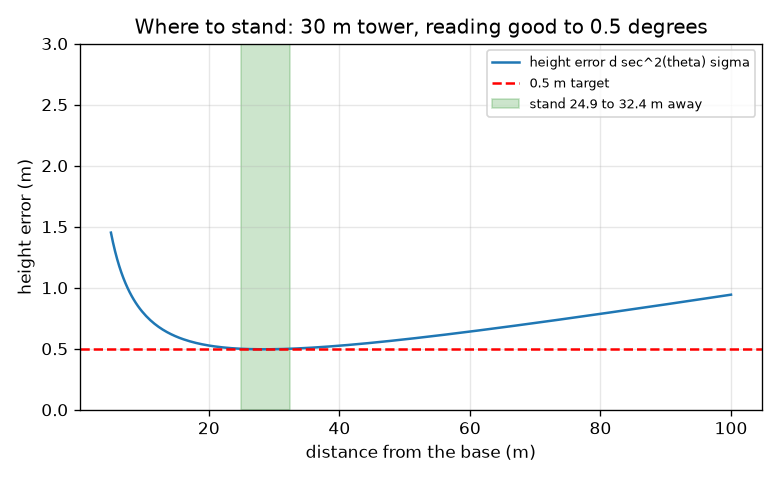
\includegraphics[width=0.85\linewidth]{figures/s02_error_vs_distance.png}\\\small Height error versus distance for a 30 m tower: a bowl with its minimum near 45 degrees; the green band meets the 0.5 m limit.\end{center}

\subsection*{E. Worked example}
(a) Two readings, 35.4 degrees at the far spot and 43.5 degrees after walking b = 10 m towards a tower, with eye height 1.6 m. Find the height. (b) For a 30 m tower (28.4 m above the eye) and a reading error of 0.5 degrees, between which distances is the error at most 0.5 m?
\begin{enumerate}[nosep]
\item (a) cot 35.4 degrees = 1.4071 and cot 43.5 degrees = 1.0538 (using cot = 1 / tan).
\item (a) H = 10 / (1.4071 - 1.0538) = 28.30 m above the eye; total = 28.30 + 1.6 = 29.90 m.
\item (b) Convert 0.5 degrees to radians: 0.008727. Need 2 H sigma / sin(2 theta) \textless{}= 0.5, so sin(2 theta) \textgreater{}= 2 x 28.4 x 0.008727 / 0.5 = 0.9913.
\item (b) 2 theta is between 82.4 and 97.6 degrees, so theta is between 41.2 and 48.8 degrees.
\item (b) d = H / tan(theta): 28.4 / tan 48.8 = 24.9 m and 28.4 / tan 41.2 = 32.4 m.
\end{enumerate}
\textbf{Answer.} (a) The tower is 29.90 m tall. (b) Stand between 24.9 m and 32.4 m from the base: the angle is then between 41 and 49 degrees and the error stays at or below 0.5 m (it equals 0.496 m at best).

\subsection*{F. Questions}
\begin{enumerate}[nosep]
\item \textbf{Conceptual.} A friend says: stand as far away as possible, then the angle is small and the error is small. Is that right for a tower of a given height? What is true and what is not?
\item \textbf{Numerical.} A 20 m tower (18.4 m above your eye) is read from 18.4 m and from 50 m, with a reading error of 0.5 degrees. Find the height error at each distance.
\item \textbf{Graph and simulation interpretation.} On the error graph for the 30 m tower (0.5 degrees), where is the minimum and what is its value? Is a 0.5 m limit reachable at 60 m?
\item \textbf{Design and optimisation challenge.} Design: the 30 m tower must be measured to within 0.5 m with a clinometer good to 0.5 degrees, but a wall means you can only stand 40 m or farther away. What can you do? Then suppose the clinometer is only good to 1 degree: what is the best possible single-reading error and what could you change?
\end{enumerate}

\section{Session 3: Simulating noisy readings, hills and averages}

\subsection*{A. Real-world problem}
A phone clinometer never gives the same angle twice. Is the error formula from Session 2 right? Does averaging many readings help, and by how much? Is the two-angle method better? What if you stand on a hill, or so close to a tall tower that you look almost straight up? And finally: how tall is the school flagpole, with an honest error bar?

\subsection*{B. Concept and theory}
A simulation starts from exact geometry: the true angle is atan(H / d). The phone adds a random error with standard deviation sigma, so the reading is the true angle plus noise, and each reading gives a height estimate. The mean of n independent estimates has standard error s / sqrt(n), where s is the sample standard deviation (with n - 1 in the denominator): averaging shrinks random error but not a systematic one such as a tilted phone. A Monte Carlo test repeats the measurement thousands of times and compares the spread of the results with the formula. The two-angle error is found by propagating both reading errors: each partial derivative of H = b / (cot a1 - cot a2) is multiplied by sigma and the two contributions are added in quadrature. On a slope with angle phi (ground rising towards the tower), a tape along the ground gives the slope distance s, the horizontal distance is D = s cos(phi), and the tower height above its base is D (tan a - tan phi) + e. Ignoring the slope gives e + s tan a, which is wrong. This is a simplified model: independent Gaussian errors, a vertical tower, a level phone and a straight slope. It is not a surveying standard.

\begin{itemize}[nosep]
\item sigma: standard deviation of one angle reading (degrees)
\item n: number of readings averaged (no unit)
\item s: sample standard deviation of the heights (m)
\item SEM: standard error of the mean, s / sqrt(n) (m)
\item phi: ground slope angle (positive rising towards the tower) (degrees)
\item s\_d, D: slope distance along the ground and horizontal distance D = s\_d cos(phi) (m)
\item b, a1, a2: walk and the two readings of the two-angle method (m, degrees)
\end{itemize}

\begin{equation*}
\hat h=d\tan(\theta_{\mathrm{true}}+\varepsilon)+e,\qquad \varepsilon\sim N(0,\sigma^2)
\end{equation*}

\begin{equation*}
\mathrm{SEM}=\frac{s}{\sqrt n}
\end{equation*}

\begin{equation*}
\sigma_H^{(1)}=d\sec^2\theta\,\sigma,\qquad \sigma_H^{(2)}=\sigma\,\frac{b\sqrt{\csc^4 a_1+\csc^4 a_2}}{(\cot a_1-\cot a_2)^2}
\end{equation*}

\begin{equation*}
h=D(\tan a-\tan\varphi)+e,\qquad D=s_d\cos\varphi
\end{equation*}

\begin{center}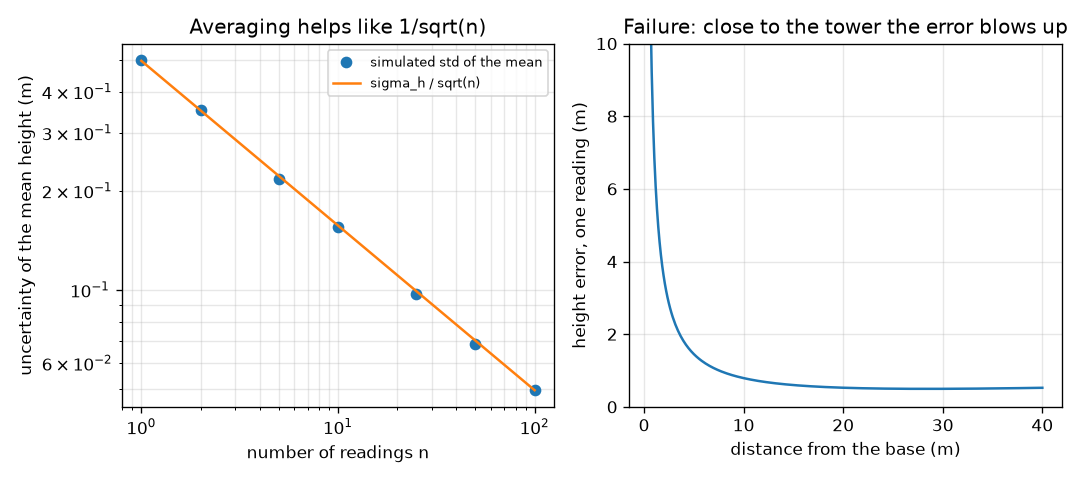
\includegraphics[width=0.85\linewidth]{figures/s03_averaging_and_failure.png}\\\small Left: averaging n readings follows 1 / sqrt(n). Right: close to the tower the single-reading error blows up.\end{center}

\subsection*{E. Worked example}
(a) A 30 m tower stands 30 m (horizontal) up a 10 degree slope from you, eye height 1.6 m. The true top angle is 48.32 degrees. Find the height ignoring the slope and with the slope correction. (b) The flagpole data (12 readings at 18.0 m, eye 1.55 m) give heights with a mean of 9.38 m and a standard error of 0.035 m. How big is the tape error contribution for a 0.1 m tape error, and what is the combined uncertainty?
\begin{enumerate}[nosep]
\item (a) Slope distance s = 30 / cos 10 degrees = 30.46 m. Ignoring the slope: 1.6 + 30.46 x tan 48.32 degrees = 35.81 m.
\item (a) With the correction: 30 x (tan 48.32 - tan 10) + 1.6 = 30 x (1.1230 - 0.1763) + 1.6 = 30.00 m.
\item (b) The tape error enters like a distance error: 0.1 m x tan(mean angle 23.5 degrees) = 0.1 x 0.4350 = 0.0435 m (angle of the mean reading).
\item (b) Combine in quadrature: sqrt(0.035\textasciicircum{}2 + 0.0435\textasciicircum{}2) = 0.056 m.
\item (b) Report: 9.38 +/- 0.06 m.
\end{enumerate}
\textbf{Answer.} (a) Ignoring the slope gives 35.81 m, wrong by 5.8 m; the correction gives the true 30.00 m. (b) The flagpole is 9.38 +/- 0.06 m (standard error 0.035 m, tape contribution 0.044 m).

\subsection*{F. Questions}
\begin{enumerate}[nosep]
\item \textbf{Conceptual.} Your phone is tilted so that every reading is 1 degree too large. Does averaging 100 readings fix it? What would?
\item \textbf{Numerical.} At 45 degrees and 28.4 m, one reading gives a height error of 0.496 m. How many readings must you average to bring the standard error to 0.1 m or below? What do you get with 25?
\item \textbf{Graph and simulation interpretation.} In the Monte Carlo results for far reading at 40 m, the one-angle standard deviation is 0.52 m while the two-angle method gives 2.64 m for a 10 m walk and 0.74 m for a 30 m walk. Explain what the graph shows and when the two-angle method is worth using.
\item \textbf{Design and optimisation challenge.} Design: a 30 m tower on a 10 degree slope, a clinometer good to 0.5 degrees, and a limit of 0.15 m on the uncertainty of the mean. Choose the horizontal distance and the number of readings. What could go wrong at 3 m?
\end{enumerate}

\section{Real-world mini-project}
\textbf{Measure your school's flagpole.} You stood 18.0 m (horizontal, by tape, good to 0.1 m) from the flagpole with your eye 1.55 m above the ground, and took 12 phone readings of the angle to the top. The synthetic readings are stored in \texttt{FLAG\_READINGS} in Session 3. Turn the 12 readings into a height with an uncertainty, using \texttt{h\_one}, \texttt{mean\_and\_sem} and the tape error.

\section{The path ahead}
\begin{enumerate}[nosep]
\item \textbf{Session 4: Calibrate the phone.} A small model of a clinometer with an offset and noise, and a calibration routine that uses readings from both sides.
\item \textbf{Session 5: Outlier-proof averaging.} An estimator that rejects outliers and still reports an uncertainty.
\item \textbf{Session 6: Measure a leaning tree.} A solver that finds the vertical height and the lean angle from readings taken from several places.
\item \textbf{Session 7: Unknown ground: three stations.} A least-squares fit of height and base position from readings at three non-collinear stations.
\item \textbf{Session 8: Animate the walk-away estimate.} A looping animation of an observer walking away from a tower with sight lines and a converging estimate.
\end{enumerate}

\section{Answers and hints}

\subsection*{Session 1}
\begin{enumerate}[nosep]
\item \textbf{Conceptual.} Hint: Similar means same angles. What sets the angle between the sun ray and the ground? Solution: At one moment the sun rays are parallel, so the angle between the sun and the flat ground is the same for stick and tower; the right angle at the ground is also shared, so all angles match and the triangles are similar. At 9 am and 11 am the sun is at different heights, so the shadow-to-height ratio differs and the answer is wrong. Measure both shadows at the same time.
\item \textbf{Numerical.} Hint: Use h\_t = h\_s s\_t / s\_s, then h = d tan a + e. tan 40 degrees = 0.8391. Solution: First tree: 2.0 x 15 / 1.2 = 25.0 m. Second tree: 12 x 0.8391 = 10.07 m above the eye, plus 1.6 m gives 11.67 m. Sanity check: at 40 degrees (a bit less than 45) the height above the eye is a bit less than the distance 12 m, so about 10 m is right.
\item \textbf{Graph and simulation interpretation.} Hint: Use the curve for d = 40 m, or compute 40 tan(a) + 1.6. Solution: At 20 degrees about 16.2 m, at 45 degrees 41.6 m, at 60 degrees 70.9 m. From 20 to 45 degrees the height gains 25.4 m (about 1.0 m per degree); from 45 to 60 it gains 29.3 m in 15 degrees (about 2.0 m per degree). The curve gets steeper because the tangent grows faster at large angles; a 1 degree slip matters more there.
\item \textbf{Design and optimisation challenge.} Hint: Compute d for an angle of 45 degrees, where tan a = 1. Think about holding the phone steady at steep angles and about the angle getting small at long distances. Solution: For 45 degrees, tan a = 1, so d = h - e = 12 - 1.6 = 10.4 m. Standing 2 m away gives an angle near 79 degrees: you look almost straight up, the phone is hard to hold, and small angle slips make large height changes (Session 2). Standing 45 m away gives only about 13 degrees, and the top is a small angle above the horizon, so a small slip is a large fraction of the reading and branches or trees may block the view. Trade-off: about 45 degrees is a good compromise, with room for obstacles.
\end{enumerate}

\subsection*{Session 2}
\begin{enumerate}[nosep]
\item \textbf{Conceptual.} Hint: Write the error as 2 H sigma / sin(2 theta) and ask what happens at small theta. Solution: For a FIXED distance d the error d sec\textasciicircum{}2(theta) sigma is smaller at smaller angles. But for a given tower you change the angle only by changing d: d = H / tan(theta), and then the error is 2 H sigma / sin(2 theta), which gets large when theta is small (sin 2 theta is small). Far away is worse: for the 30 m tower the error at 100 m is 0.94 m against 0.50 m at 28.4 m.
\item \textbf{Numerical.} Hint: At 18.4 m the angle is 45 degrees. For 50 m find the angle from tan(theta) = 18.4 / 50, then use d sec\textasciicircum{}2(theta) sigma. Solution: At 18.4 m, theta = 45 degrees: error = 2 x 18.4 x 0.008727 = 0.32 m. At 50 m, theta = atan(18.4 / 50) = 20.2 degrees and sec\textasciicircum{}2 = 1 + (18.4 / 50)\textasciicircum{}2 = 1.135, so error = 50 x 1.135 x 0.008727 = 0.50 m. The farther position is about 1.5 times worse. Units: metres.
\item \textbf{Graph and simulation interpretation.} Hint: Read the bottom of the bowl and compare the curve at 60 m with the red line. Solution: The minimum is at 28.4 m, where the angle is 45 degrees, and equals about 0.50 m. At 60 m the error is 0.64 m, above the red 0.5 m line, so a single reading from 60 m cannot meet the limit. Only the window 24.9 m to 32.4 m meets it.
\item \textbf{Design and optimisation challenge.} Hint: Compute the best single-reading error 2 H sigma for sigma = 0.5 and 1 degree. Think about what independent repeats do to a random error (Session 3). Solution: At 40 m the single-reading error is 0.525 m, just above the limit, so one reading is not enough; the practical option is to repeat the reading several times and average (random error falls as 1 / sqrt(n), Session 3). With sigma = 1 degree even the best spot gives 2 x 28.4 x 0.01745 = 0.99 m, so one reading can never meet 0.5 m; averaging n \textgreater{}= (0.99 / 0.5)\textasciicircum{}2 = 3.9, so at least 4 independent readings, would. Trade-off: more readings cost time, and averaging does not remove a tilted-phone bias.
\end{enumerate}

\subsection*{Session 3}
\begin{enumerate}[nosep]
\item \textbf{Conceptual.} Hint: Compare random and systematic errors, and what the standard error measures. Solution: No. The standard error measures the random scatter, which falls as 1 / sqrt(n), but a constant offset shifts the mean by the same amount however many readings you take. The bias at 45 degrees and 28.4 m is 28.4 x 2 x 0.01745 = 0.99 m. Calibrate the phone first (for example against a known horizontal), or measure the same known height and correct the offset.
\item \textbf{Numerical.} Hint: SEM = sigma\_H / sqrt(n); solve for n and round up. Solution: n \textgreater{}= (0.496 / 0.1)\textasciicircum{}2 = 24.6, so n = 25. With 25 readings the standard error is 0.496 / 5 = 0.099 m, matching the simulation (0.097 m). Sanity check: sqrt(25) = 5, so 25 readings make the error 5 times smaller than one reading.
\item \textbf{Graph and simulation interpretation.} Hint: The two-angle method subtracts two cotangents that are nearly equal when the walk is short. Solution: A short walk makes cot a1 - cot a2 small, so the angle errors are divided by a small number squared and amplified. A longer walk improves it but one-angle with a known distance stays better (0.52 m at 40 m). Use the two-angle method only when you cannot measure the distance to the base, and then walk as far as you can: the 30 m walk gives 0.74 m.
\item \textbf{Design and optimisation challenge.} Hint: The best distance puts the top angle near 45 degrees; the top is 28.4 + D tan(10 degrees) above your eye. Solution: The top angle is 45 degrees when D = 28.4 + D tan 10, so D = 28.4 / (1 - 0.1763) = 34.5 m; take D = 35 m. One reading gives about 0.60 m, so n \textgreater{}= (0.60 / 0.15)\textasciicircum{}2 = 16; with n = 25 the uncertainty is 0.12 m. At 3 m the top angle is about 84 degrees and the single-reading error is 2.5 m: you are in the failure region, and a reading near 90 degrees also has a large bias (for example a bias of +0.4 m at 2 m from the tower on flat ground). Trade-off: more readings take time and cannot fix a slope angle you did not measure.
\end{enumerate}

\section{How to join}
Read \texttt{CONTRIBUTING.md} in the repository, then pick an issue labelled \texttt{good first issue}. Repository: \url{https://github.com/KrunalPanchal1995/openheights}

\end{document}
